\begin{multicols}{2}
	\begin{center}
		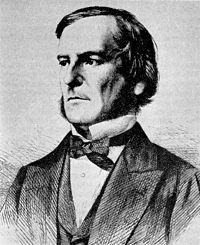
\includegraphics[height=.8\textheight]{./IMG/boole.jpg}
	\end{center}

\vfill
\columnbreak

\begin{itemize}
	\item 1849: “Análise Matemática da Lógica”
	\item Álgebra de Boole
	\item Álgebra booleana
\end{itemize}

"[...] É com base nesse princípio geral que eu pretendo estabelecer o \textbf{cálculo da lógica, e que reivindico para ele um lugar entre as formas reconhecidas da análise matemática}."

\vfill\null
\columnbreak
{\large \textbf{FALSO}\\
0\\
NÃO\\
DESLIGADO
}


\begin{center}
	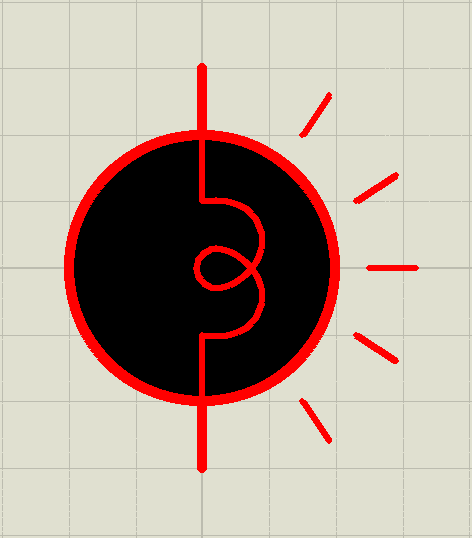
\includegraphics[height=.7\textheight]{./IMG/FALSO.png}
\end{center}

\vfill
\columnbreak

{\large \textbf{VERDADEIRO}\\	
	1\\	
	SIM\\	
	LIGADO\
}

\begin{center}

	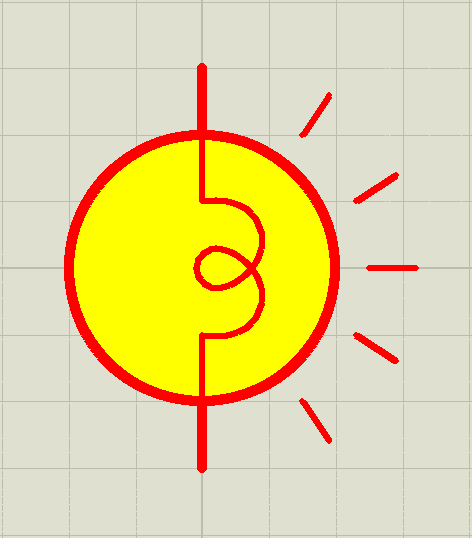
\includegraphics[height=.7\textheight]{./IMG/VERDADEIRO.png}
\end{center}

\vfill
\columnbreak

\begin{center}
	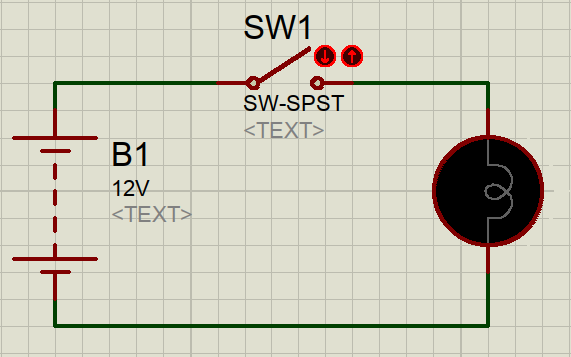
\includegraphics[width=.9\linewidth]{./IMG/Screenshot_20231216_190844.png}
\end{center}

\vfill
\columnbreak

\begin{center}
	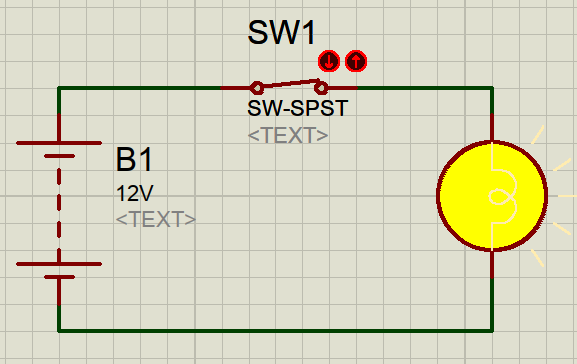
\includegraphics[width=.9\linewidth]{./IMG/Screenshot_20231216_191027.png}
\end{center}
\end{multicols}



\begin{table}[h]
	\centering
	\Large
	\caption{\textbf{Tabela Verdade}}
	\begin{tabular}{|>{\centering\arraybackslash}p{.125\textwidth}|>{\centering\arraybackslash}p{.125\textwidth}|}
		\hline
		\textbf{Botão} & \textbf{Lâmpada} \\
		\hline
		\textbf{0} & \textbf{0} \\
		\hline
			\textbf{1} & \textbf{1} \\
		\hline
	\end{tabular}
\end{table}




\vfill
\pagebreak

\begin{multicols}{3}


\begin{center}
	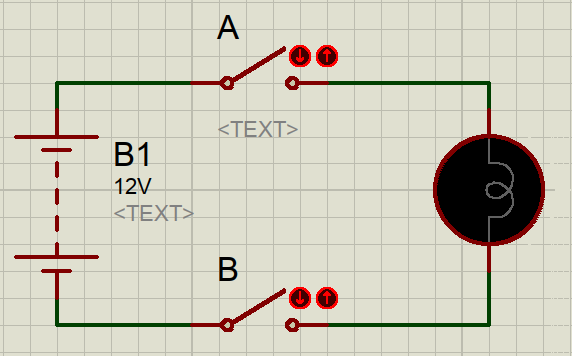
\includegraphics[width=\linewidth]{./IMG/Screenshot_20231216_191616.png}
\end{center}

 
 \begin{center}
 	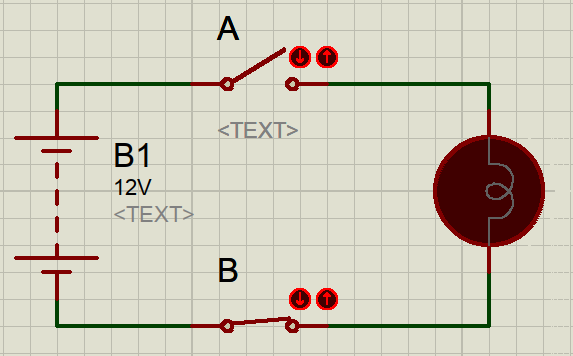
\includegraphics[width=\linewidth]{./IMG/Screenshot_20231216_191707.png}
 \end{center}

\vfill\null
\columnbreak

\begin{center}
	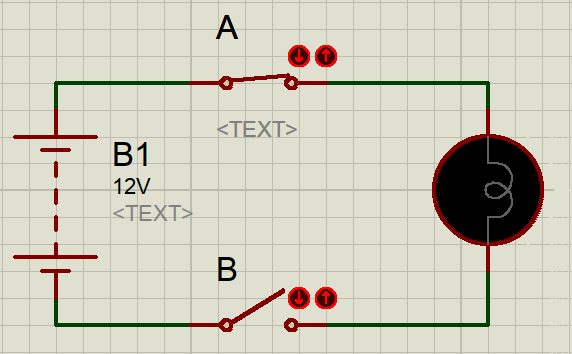
\includegraphics[width=\linewidth]{./IMG/Screenshot_20231216_191640.png}
\end{center}

\begin{center}
	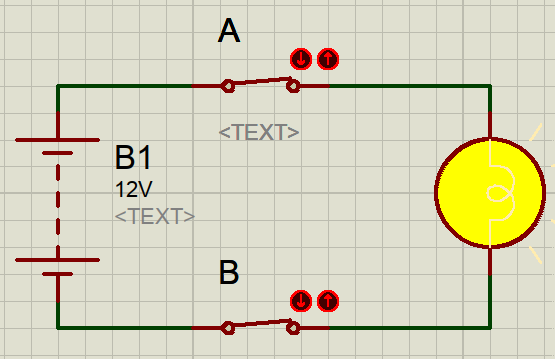
\includegraphics[width=\linewidth]{./IMG/Screenshot_20231216_191745.png}
\end{center}

\vfill\null
\columnbreak

 \centering
\begin{tabular}{|>{\centering\arraybackslash}p{.25\linewidth}|>{\centering\arraybackslash}p{.25\linewidth}|>{\centering\arraybackslash}p{.25\linewidth}|}
	\hline
	A & B & L\\
	\hline
	0 & 0 & 0 \\
	\hline
	1 & 0 & 0 \\
	\hline
	0 & 1 & 0 \\
	\hline
	1 & 1 & 1 \\
	\hline
\end{tabular}

\vfill\null
\columnbreak

\begin{center}
	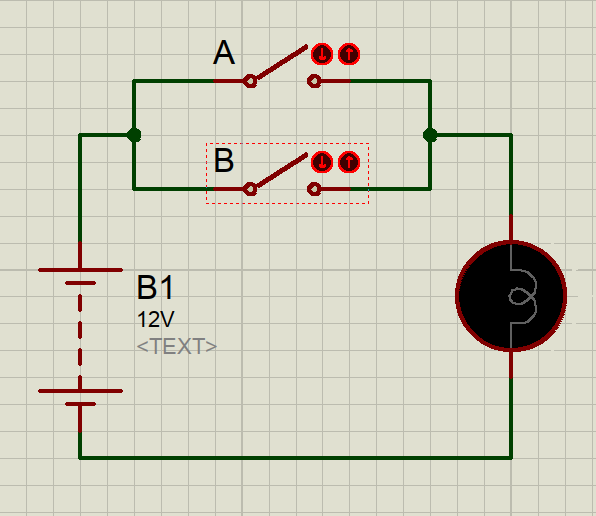
\includegraphics[width=.8\linewidth]{./IMG/Screenshot_20231216_192237.png} 
\end{center}
   
\begin{center}
	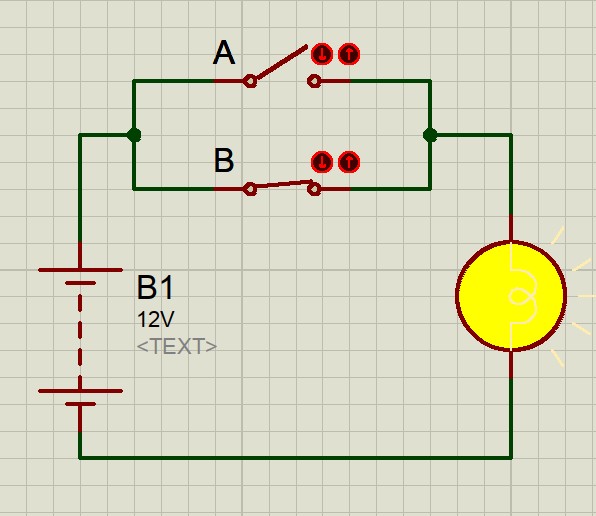
\includegraphics[width=.8\linewidth]{./IMG/Screenshot_20231216_192323.png}
\end{center}

\vfill
\columnbreak
 
\begin{center}
	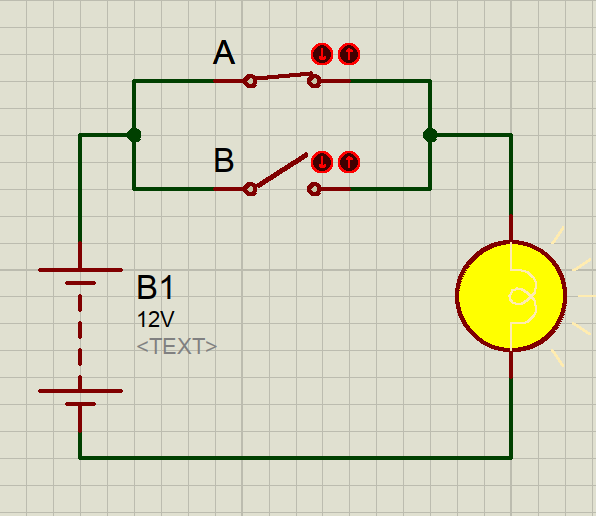
\includegraphics[width=.8\linewidth]{./IMG/Screenshot_20231216_192257.png}
\end{center}
    
\begin{center}
	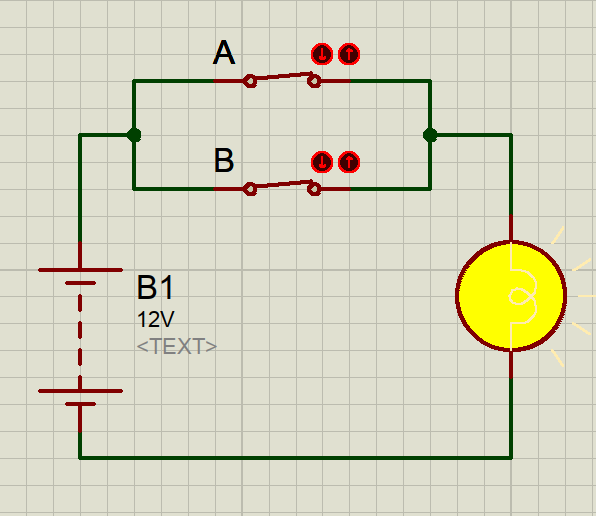
\includegraphics[width=.8\linewidth]{./IMG/Screenshot_20231216_192355.png}
\end{center}

\vfill
\columnbreak

 \centering
\begin{tabular}{|>{\centering\arraybackslash}p{.25\linewidth}|>{\centering\arraybackslash}p{.25\linewidth}|>{\centering\arraybackslash}p{.25\linewidth}|}
	\hline
	A & B & L\\
	\hline
	0 & 0 & 0 \\
	\hline
	1 & 0 & 1 \\
	\hline
	0 & 1 & 1 \\
	\hline
	1 & 1 & 1 \\
	\hline
\end{tabular}


\end{multicols}

\vfill
\pagebreak